\chapter{CuS--MoS$_2$ Reinforcement Within PVA Matrix}\label{ch:cusmos2}

This chapter emphasizes that CuS--MoS$_2$ is a dispersed nanofiller network inside PVA. The continuous scaffold remains PVA.

\section{Heterostructure Synergy and Band Alignment}
CuS and MoS$_2$ can form a heterointerface aiding charge transfer and interfacial polarization. A qualitative band offset descriptor is
\begin{equation}\label{eq:band_offset}
\Delta E_C=\chi_{MoS_2}-\chi_{CuS},\qquad \Delta E_V=E_{g,CuS}-E_{g,MoS_2}+\Delta E_C.
\end{equation}

\section{Percolation Threshold Modeling}
Electrical conductivity near percolation is approximated by
\begin{equation}\label{eq:percolation}
\sigma_{eff}=\sigma_m + A(\phi_f-\phi_c)^t\,H(\phi_f-\phi_c),
\end{equation}
where $\phi_f$ is filler loading, $\phi_c$ threshold, and $H$ the Heaviside function.

\section{Effective Medium Theory}
Maxwell--Garnett estimate for dilute fillers:
\begin{equation}\label{eq:mg}
\frac{k_{eff}-k_m}{k_{eff}+2k_m}=\phi_f\frac{k_f-k_m}{k_f+2k_m}.
\end{equation}
Bruggeman symmetric relation for higher loadings:
\begin{equation}\label{eq:bruggeman}
\phi_f\frac{k_f-k_{eff}}{k_f+2k_{eff}}+(1-\phi_f)\frac{k_m-k_{eff}}{k_m+2k_{eff}}=0.
\end{equation}

\section{Interfacial Resistance and Phonon Scattering}
Kapitza resistance contributes to reduced effective conduction:
\begin{equation}\label{eq:kapitza}
\Delta T_{int}=q''R_K.
\end{equation}
Nanofiller interfaces raise boundary scattering rates:
\begin{equation}\label{eq:phonon_boundary}
\ell_{ph,eff}^{-1}=\ell_{ph,bulk}^{-1}+\beta\frac{\phi_f}{d_f}.
\end{equation}

\begin{figure}[htbp]
\centering
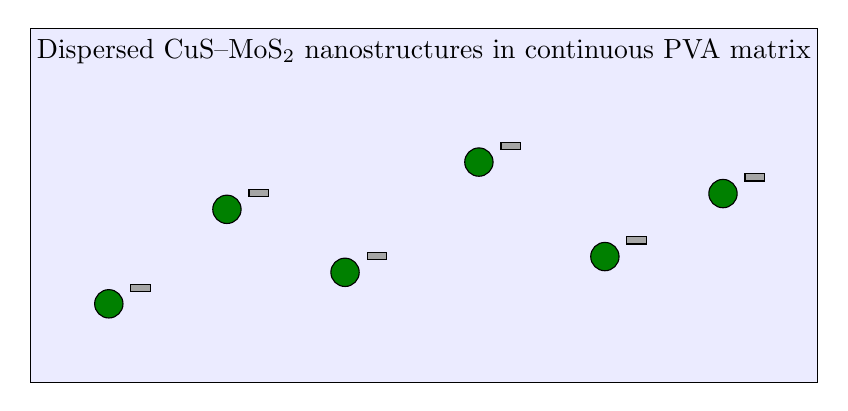
\begin{tikzpicture}
\draw[fill=blue!8] (0,0) rectangle (10,4.5);
\foreach \x/\y in {1/1,2.5/2.2,4/1.4,5.7/2.8,7.3/1.6,8.8/2.4}{
\draw[fill=green!50!black] (\x,\y) circle (0.18);
\draw[fill=gray!70] (\x+0.28,\y+0.16) rectangle +(0.25,0.09);
}
\node at (5,4.2) {Dispersed CuS--MoS$_2$ nanostructures in continuous PVA matrix};
\end{tikzpicture}
\caption{Schematic of CuS--MoS$_2$ reinforcement as nanofillers within PVA (not scaffold replacement).}
\label{fig:cusmos2_dispersion}
\end{figure}

\begin{table}[htbp]
\centering
\caption{Nanofiller-reinforcement parameters for modeling.}
\label{tab:cusmos2_params}
\begin{tabular}{lcc}
\toprule
Parameter & Symbol & Range \\
\midrule
Filler fraction & $\phi_f$ & 0.5--8 vol\% \\
Percolation threshold & $\phi_c$ & 1--3 vol\% \\
Kapitza resistance & $R_K$ & $10^{-8}$--$10^{-6}$ \si{\meter\squared\kelvin\per\watt} \\
Aspect ratio & $a_r$ & 5--30 \\
\bottomrule
\end{tabular}
\end{table}

\begin{table}[htbp]
\centering
\caption{Expected reinforcement effects at moderate loading.}
\label{tab:cusmos2_effects}
\begin{tabular}{lcc}
\toprule
Property & Baseline PVA/PCM & With CuS--MoS$_2$ reinforcement \\
\midrule
$\sigma_{eff}$ & low & moderate-to-high \\
$k_{eff}$ & low & controlled increase \\
Cycle modulus retention & moderate & improved \\
Agglomeration risk & negligible & rises above optimal loading \\
\bottomrule
\end{tabular}
\end{table}
